\documentclass[spanish]{article}
\usepackage[a4paper, left=1in, right=1in, top=1in, bottom=1in]{geometry}
                                % for page size and margin settings
\usepackage{graphicx}		    % for insert images
\usepackage[es-tabla]{babel} 	% for spanish titles
\usepackage[a4paper, left=1in, right=1in, top=1in, bottom=1in]{geometry} 
								% for page size and margin settings
\usepackage{mathtools}          % for greek math symbol formatting
\usepackage{enumitem}           % for control of 'enumerate' numbering
\usepackage{listings}           % for control of 'itemize' spacing
\usepackage{indentfirst}		% package to make first paragraph always indented
\usepackage{hyperref}           % page numbers and '\ref's become clickable
\usepackage{bm}					% for bold maths
\usepackage{setspace}			% for setting interline spacing
\usepackage{amsmath}			% for matrices
\usepackage{tikz} 				% for graphs
\usepackage{multirow}			% for tables
\usepackage{float}				% to manually select placement of tables

\usetikzlibrary{babel}		    % for draw arrows in tikz using babel spanish
\renewcommand{\baselinestretch}{1.5}
\bibliographystyle{ieeetr}
\numberwithin{figure}{subsection}
\numberwithin{equation}{subsection}
\numberwithin{table}{subsection}

% TITLE VARIABLES 

\def\thesistitle{Incorporación de covariables que varían en el tiempo a un modelo mixto}
\def\thesisauthorfirst{\textbf{Esteban Cometto}}
\def\thesissupervisorfirst{Noelia Castellana}
\def\thesissupervisorsecond{Cecilia Rapelli}
\def\thesisdate{\today}

%% OTHER USEFUL VARIABLES 

\def\npatients{560}
\def\fullcovname{adherencia al tratamiento farmacológico}
\def\covname{\textit{adherencia}}
\def\cvt{covariable que varía en el tiempo}
\def\xseqj{$X_{i1}, ..., X_{ij}$}
\def\xseqn{$X_{i1}, ..., X_{in_i}$}
\def\xseqjminus{$X_{i1}, ..., X_{ij-1}$}
\def\yseqj{$Y_{i1}, ..., Y_{ij}$}
\def\yseqn{$Y_{i1}, ..., Y_{in_i}$}
\def\yseqjminus{$Y_{i1}, ..., Y_{ij-1}$}

%% FOR PDF METADATA
\title{\thesistitle}
\author{\thesisauthorfirst\space\thesisauthorsecond}
\date{\thesisdate}

\begin{document}

\begin{titlepage}
    \newcommand{\HRule}{\rule{\linewidth}{0.5mm}}
	\center
	\textsc{\Large Universidad Nacional de Rosario}\\[.7cm]
	
\includegraphics[width=25mm]{img/fceye-unr.png}\\[.5cm]
	\textsc{Facultad de Ciencias Económicas y Estadística}\\[0.5cm]
	\textsc{Anteproyecto de Tesina}
	
	\HRule \\[0.4cm]
	{ \huge \bfseries \thesistitle}\\[0.1cm]
	\HRule \\[.5cm]
	
	\begin{minipage}{0.6\textwidth}
	\large
	\textit{Autor:}	\thesisauthorfirst
	\end{minipage}
	\\[.6cm]
	\begin{minipage}{0.6\textwidth}
	\textit{Directora:} 	\thesissupervisorfirst \\[.2cm]
	\textit{Codirectora:} 	\thesissupervisorsecond
	\end{minipage}
	\\[4cm]
	\vfill
	{\large \thesisdate}\\
	\clearpage
\end{titlepage}

\newpage
\tableofcontents

\newpage
\section{Introducción}

Los datos longitudinales tienen la particularidad de estar conformados por
mediciones repetidas sobre una unidad, las cuales pueden surgir por ser medidas
en diferentes momentos o conidiciones. Su principal interés es estudiar los
cambios en el tiempo y los factores que influencian el cambio. 

Los modelos mixtos permiten ajustar datos con estas particularidades, donde la
respuesta es modelada por una parte sistemática que está formada por una
combinación de características poblacionales que son compartidas por todas las
unidades (efectos fijos), y una parte aleatoria que está constituida por
efectos específicos de cada unidad (efectos aleatorios) y por el error
aleatorio.

Las covariables en los estudios longitudinales se pueden clasificar en dos
categorias: fijas y variables en el tiempo. Las diferencias entre estos tipos
de covariables pueden llevar a diferentes intereses de investigación,
diferentes tipos de análisis y diferentes conclusiones.

Las covariables fijas son variables independientes que no tienen variación
intra-sujeto, lo que significa que el valor de la covariable no cambia para un
individuo determinado en el estudio longitudinal. Este tipo de covariable se
puede usar para realizar comparaciones entre poblaciones y describir diferentes
tendencias en el tiempo, pero no permite una relación dinámica entre la
covariable y la respuesta.

Las covariables variables en el tiempo (CVT) son variables independientes que
contienen ambas variaciones, intra y entre sujeto, lo que significa que el
valor de la covariable cambia para un individuo determinado a lo largo del
tiempo y además puede cambiar para diferentes sujetos. Una CVT se puede usar
para hacer comparaciones entre poblaciones, describir tendencias en el tiempo y
también la relación dinámica entre la CVT y la respuesta

Se puede ver que las CVT permiten diferentes tipos de relaciones y conclusiones
que las covariables fijas. Por ejemplo, covariables como la edad pueden cambiar
a través del tiempo, pero cambian de manera predecible. Por otro lado,
covariables como la precipitación diaria pueden cambiar a través del tiempo
pero no pueden ser predecidas. En esos casos es importante considerar las
relaciones entre la CVT y la respuesta a través del tiempo.

En el presente informe se cuenta con un programa de atención y control de
pacientes hipertensos iniciado en el año 2014 en Rosario. En cada visita se
registra el seguimiento del tratamiento y los valores de la tensión arterial
sistólica. En particular, se desea evaluar si la adherencia al tratamiento
farmacológico influye en los valores de la tensión arterial sistólica (TAS) a
lo largo del seguimiento. Como la variable “\fullcovname{}” es una CVT
estocástica se evaluaran diferentes enfoques para incluirla en un modelo
longitudinal que pueda explicar el cambio en la tensión arterial sistólica
media a lo largo del tiempo.

%%%%%%%%
% ESTO QUIZAS CONVIENE PONERLO EN LOS RESULTADOS
%%%%%%%%
%%%%%%%%
% ESTO QUIZAS CONVIENE PONERLO EN LOS RESULTADOS
%%%%%%%%
%%%%%%%%
% ESTO QUIZAS CONVIENE PONERLO EN LOS RESULTADOS
%%%%%%%%

Un aspecto a tener en cuenta en este trabajo es que, si bien contamos con mucha
otra información para obtener modelos que describan de mejor manera el
comportamiento de la TAS, nos centraremos en modelos más simples con respecto a
las covariables fijas con el fin de no perder de vista la relación entre la
variable respuesta y la CVT.

\newpage
\section{Objetivos}

\subsection{Objetivo Principal}

Presentar diferentes propuestas metodológicas respecto a la incorporación de
covariables que varían con el tiempo en modelos mixtos para datos
longitudinales.

\subsection{Objetivos Específicos}

\begin{itemize}
	\item Definir los tipos de covariables existentes.
	\item Evaluar propuestas de incorporación de covariables que varían en el
	tiempo en los modelos mixtos.
	\item Aplicar los conceptos vistos en un estudio sobre la tendencia de la
		  presión arterial en el tiempo para pacientes que siguen cierto
		  tratamiento.
\end{itemize}

\newpage
\section{Los Datos Longitudinales}

Los datos longitudinales están conformados por mediciones repetidas de una
misma variable realizadas a la misma unidad. Estas mediciones surgen de
observar unidades en diferentes ocasiones, es decir en diferentes momentos o
condiciones experimentales.

Dado que las mediciones repetidas son obtenidas de la misma unidad, los datos
longitudinales están agrupados. Las observaciones dentro de un mismo
agrupamiento generalmente están correlacionadas positivamente. Por lo tanto,
los supuestos usuales acerca de la independencia entre las respuestas de cada
unidad y la homogeneidad de variancias frecuentemente no son válidos

Las ocasiones en las que se registran las mediciones repetidas no
necesariamente serán iguales para todos los individuos, por lo tanto se pueden
obtener tanto estudios balanceados (todos los individuos tienen el mismo número
de mediciones durante un conjunto de ocasiones comunes) como desbalanceados (la
secuencia de tiempos de observaciones no es igual para todos los individuos).
Otra característica de estos datos es que en ocasiones se pueden obtener
valores perdidos, obteniendo datos incompletos aunque se cuente con un estudio
balanceado.

Con el fin de simplificar la notación, se asumirá que los tiempos de medición
son los mismos para todas las unidades y que no hay datos faltantes.

Se obtiene una muestra de $N$ unidades cada una con $n$ mediciones repetidas de
la variable en estudio, observadas en los tiempos $t_1, t_2, ..., t_n$, siendo
entonces el número total de observaciones $N^*=Nn$. Se le llama $Y_{ij}$ a la
medición sobre la unidad $i$ en la ocasión $j$, con $i=1, ..., N; j=1, ..., n$

Asociadas a cada unidad se observan las covariables $X_{ij}$ medidas también
sobre la unidad $i$ en la ocasión $j$. Se asume que $Y_{ij}$ y $X_{ij}$ son
simultáneamente medidas. Esto quiere decir que en un análisis de corte
transversal, $Y_{ij}$ y $X_{ij}$ se correlacionan directamente. Sin embargo,
para un análisis longitudinal se debe asumir que existe un orden
pre-establecido:
$(X_{i1}, Y_{i1}), (X_{i2}, Y_{i2}), ..., (X_{in_i}, Y_{in_i})$


Existen tres fuentes potenciales de variabilidad que influyen sobre la
correlación entre medidas repetidas:

\begin{itemize}
	\item \textit{Heterogeneidad entre las unidades:} Refleja la propensión
	natural de las unidades a responder. Los individuos tienen diferentes
	reacciones frente a los mismos estímulos.
	\item \textit{Variación biológica intra-unidad:} Se piensa que la secuencia
	de medidas repetidas de una unidad tiene un comportamiento determinado, que
	produce que las mediciones más cercanas sean más parecidas.
	\item \textit{Error de medición:} Surge debido a los errores de medida, se
	puede disminuir usando instrumentos de medición más precisos
\end{itemize}

Estas tres fuentes de variación pueden clasificarse en \textit{``variabilidad
entre''}, es decir, la variación entre las unidades (heterogeneidad entre
unidades) y \textit{``variabilidad intra''}, es decir, la variación entre las
mediciones de las misma unidad (variación biológica intra-unidad y error de
medición)

Dado que, como se mencionó anteriormente, las mediciones están correlacionadas
entre sí, si se utilizaran las técnicas habituales basadas en la independencia
entre mediciones, los errores estándares nominales van a ser incorrectos, lo
cual nos llevaría a inferencias incorrectas sobre los parámetros del modelo. En
base a esto, surgen técnicas que consideran esa correlación modelando los datos
considerando la modelación de dos estructuras: la parte media y la estructura
de covariancia.

\section{Modelos lineales mixtos}

En estos modelos, cada unidad tiene una trayectoria individual caracterizada
por parámetros y un subconjunto de esos parámetros ahora se consideran
aleatorios. La respuesta media es modelada como una combinación de
características poblacionales que son comunes a todos los individuos (efectos
fijos) y efectos específicos de la unidad que son únicos de ella (efectos
aleatorios).

Se consideran las dos fuentes de variación (intra y entre) presentes en los
datos longitudinales. Entonces, este modelo va a ser similar al modelo lineal
general con respecto a la parte media del mismo, pero se va a diferenciar en
cuanto a la estructura de covariancia.

El modelo lineal mixto para la unidad $i$ se puede expresar en forma matricial
como:

\[ Y_i = X_i\beta + Z_ib_i + \varepsilon_i; \quad i = 1, ..., N;
\quad Y_i = (Y_{i1}, Y_{i2}, ... Y_{in_{i}})' \]

Donde:

\begin{itemize}
	\item $Y_i$: Vector de la variable respuesta de la i-ésima unidad, de
	dimensión $(n_i*1)$
	\item $X_i$: Matriz de diseño de la i-ésima unidad, que caracteriza la
	parte sistemática de la respuesta, de dimensión $(n_i*p)$
	\item $\beta$: Vector de parámetros de dimensión $(p*1)$
	\item $Z_i$: Matriz de diseño de la i-ésima unidad, que caracteriza la
	parte aleatoria de la respuesta, de dimensión $(n_i*k)$
	\item $b_i$: Vector de efectos aleatorios de la i-ésima unidad, de
	dimensión $(k*1)$
	\item $\varepsilon_i$: Vector de errores aleatorios de la i-ésima unidad,
	de dimensión $(n_i*1)$
\end{itemize}

$\varepsilon_i$ y $b_i$ son independientes.

\[ \varepsilon_i \sim N_{n_i}(0, R_i) \]
\[ b_i \sim N_k(0, D_i) \]

Las matrices $D_i$ y $R_i$ contienen las variancias y covariancias de los
elementos de los vectores $b_i$ y $\varepsilon_i$ respectivamente. A partir de
este modelo se obtiene:

\begin{itemize}
	\item $E(y_i/b_i) = X_i\beta + Z_ib_i$ (media condicional o específica de
	la i-ésima unidad)
	\item $E(Y_i) = X_i\beta$ (media marginal)
	\item $Cov(Y_i/b_i) = R_i$ (variancia condicional)
	\item $Cov(Y_i) = Z_iD_iZ'_i + R_i = \varSigma_i$ (variancia marginal)
\end{itemize}

Generalmente, la matriz $D_i$ adopta una estructura de covariancia arbitraria,
mientras que la matriz $R_i$ adopta cualquiera de las vistas anteriormente

\subsection{Estimación de los parámetros del modelo}

Bajo el supuesto de que $\varepsilon_i$ y $b_i$ se distribuyen normalmente se
pueden usar métodos de estimación basados en la teoría de máxima verosimilitud,
cuya idea es asignar a los parámetros el valor más probable en base a los datos
que fueron observados. Se usarán para estimar los parámetros de la parte media
y los de las estructuras de covariancia los métodos de máxima verosimilitud
(ML) y máxima verosimilitud restringida (REML) respectivamente

\subsubsection{Método de máxima verosimilitud (ML)}

Bajo el supuesto de que $Y_i \sim N_{n_i}(X_i\beta, \varSigma_i)$ y las $Y_i$
son independientes entre sí, se obtiene la siguiente función de
log-verosimilitud:

\begin{equation}
\label{ML}
	l = -\frac{1}{2} \sum_{i=1}^{N}n_i ln(2\pi) - \frac{1}{2}ln|\varSigma_i| -
	\frac{1}{2} \sum_{i=1}^{N} [(Y_i - X_i\beta)'
	\varSigma_i^{-1} (Y_i - X_i\beta)]
\end{equation}

Siendo $\varSigma_i$ función del vector $\theta$ que contiene los parámetros de
covariancia.

La ecuación anterior se debe derivar con respecto a $\beta$ y $\theta$ y luego
debe igualarse a cero, de esta manera se obtienen sus estimadores. Cuando
$\theta$ es desconocido (lo que generalmente sucede) se obtiene una ecuación no
lineal, por lo que no se puede obtener una expresión explícita de
$\hat{\theta}$, para encontrar su solución se recurren a algoritmos numéricos.
El estimador del vector $\beta$ resulta:

\[ \hat{\beta} = (\sum_{i=1}^{N} X_i'\hat{\varSigma_i}^{-1}X_i)^{-1}
\sum_{i=1}^{N} X'_i\hat{\varSigma_i}^{-1}Y_i \]

El estimador $\hat{\beta}$ resulta insesgado de $\beta$. Cuando $\theta$ es
conocido se conoce la distribución exacta del estimador. Sin embargo, cuando es
desconocido, no se puede calcular de manera exacta la matriz de covariancias de
$\hat{\beta}$. Si el número de unidades es grande se puede demostrar que
asintóticamente:

\[ \hat{\beta} \sim N_p(\beta, V_{\beta}) \quad donde \quad V_{\beta} =
(\sum_{i=1}^{N} X'_i\hat{\varSigma_i}^{-1}X_i)^{-1} \]

\subsubsection{Método de máxima verosimilitud restringida (REML)}

El inconveniente que posee el método de MV es que los parámetros de covariancia
resultan sesgados. Es decir, a pesar de que la estimación de $\beta$ resulta
insesgada, no pasa lo mismo con $\theta$. Si el tamaño de muestra es chico, los
parámetros que representan las variancias van a ser demasiado pequeños, dando
así una visión muy optimista de la variabilidad de las mediciones, es decir, se
subestiman los parámetros de covariancia. El sesgo se debe a que en la
estimación MV no se tiene en cuenta que $\beta$ es estimado a partir de los
datos.

El método REML separa la parte de los datos usada para estimar $\beta$ de
aquella usada para estimar los parámetros de $\varSigma_i$, la función de
log-verosimilitud restringida que se propone es:

\begin{equation}
\label{REML}
	l^* = -\frac{1}{2} \sum_{i=1}^{N}n_i ln(2\pi) - \frac{1}{2}ln|\varSigma_i| -
	\frac{1}{2} \sum_{i=1}^{N} [(Y_i - X_i\beta)'
	\varSigma_i^{-1} (Y_i - X_i\beta)] -
	- \frac{1}{2} ln |\sum_{i=1}^{N} X'_i \hat{\varSigma_i^{-1} X_i}|
\end{equation}

Maximizando esta funcion con respecto a $\beta$ y $\theta$ se obtiene:

\[ \hat{\beta} = (\sum_{i=1}^{N} X'_i \hat{\varSigma}_i^{-1} X_i)^{-1}
\sum_{i=1}^{N} X'_i \hat{\varSigma}_i^{-1} Y_i\]

Donde $\hat{\varSigma}_i$ es el estimador REML de ${\varSigma_i}$

\subsubsection{Problemas con la estimación}

Pepe y Anderson (1994) mostraron que estas ecuaciones llegan a cero solo si la
data cumple con el supuesto

\begin{equation}
\label{estimation_issue}
	E[Y_{ij} | X_{ij}] = E[Y_{ij} | X_{ij}, j = 1, ..., T]
\end{equation}

Esto quiere decir que la media condicional de la variable respuesta en una
determinada ocasión, dados todos los valores de la covariable, depende solo del
valor de la covariable en esa ocasión. Este supuesto se cumple tanto con
covariables no variables del tiempo como con covariables variables en el tiempo
no estocáticas. Sin embargo, para las CVT estocásticas puede no necesariamente
cumplirse: valores anteriores o posteriores de la CVT pueden confundir la
relacion entre la variable respuesta y la CVT en una determinada ocasión. En
consecuencia, esto puede conducir a estimaciones sesgadas de los efectos fijos
del modelo.

Frente a este escenario, varios autores recomendaron plantear el modelo
longitudinal marginal y realizar las estimaciones mediante GEE (ecuaciones de
estimación generalizadas) con estructura de correlación independiente o bien
utilizar el GMM (método generalizado de los momentos), donde es posible
incorporar información sobre la naturaleza de la CVT que se está analizando.

\newpage

\section{Covariables en datos longitudinales}

En los estudios longitudinales, las variables independientes pueden ser
clasificadas en dos categorías: covariables fijas, es decir que no varían en el
tiempo (CNVT) o covariables que varían en el tiempo (CVT). La diferencia entre
ellas puede conducir a diferentes enfoques de análisis así como también a
diferentes conclusiones.

Tanto las CNVT y las CVT ueden ser utilizadas para realizar comparaciones entre
poblaciones y describir diferentes tendencias a lo largo del tiempo. Sin
embargo, sólo las CVT permiten describir una relación dinámica entre la
covariable y la variable respuesta.

\subsection{Covariables fijas}

Las CNVT son variables independientes que no presentan variación intra-sujeto,
es decir, los valores de estas covariables no cambian a lo largo del estudio
para un individuo en particular.

Éstas covariables pueden ser fijas por naturaleza (por ejemplo, el sexo
biológico de una persona o el grupo de tratamiento) o pueden ser covariables
basales (es decir, medidas al inicio del estudio). Las covariables basales son
fijas por definición pero pueden ser variables en el tiempo por naturaleza, por
ejemplo, la edad varia en el tiempo pero la edad basal es fija.

\subsection{Covariables variables en el tiempo}

Las CVT son variables independientes que incluyen tanto la variación
intra-sujeto como la variación entre-sujetos. Esto significa que, para un
individuo en particular, el valor de la covariable cambia a través del tiempo y
puede cambiar también entre diferentes individuos. Por ejemplo, valor de la
presión arterial o condición de fumar (si/no).

\subsubsection{Covariables estocásticas y no estocásticas}

Las CVT no estocásticas son covariables que varían sistemáticamente a través
del tiempo pero son fijas por diseño del estudio o bien su valor puede
predecirse. En cambio, las CVT estocásticas son covariables que varían
aleatoriamente a través del tiempo, es decir, los valores en cualquier ocasión
no pueden ser estimados ya que son gobernados por un mecanismo aleatorio.
Ejemplos de las primeras son: tiempo desde la visita basal, edad, grupo de
tratamiento en los estudios cross-over. Ejemplos de las segundas son: valor del
colesterol, ingesta de alcohol (si/no), ingesta de grasas, etc.

\subsubsection{Covariables exógenas y endógenas}

Se dice que una CVT es exógena cuando los valores actuales y anteriores de la
respuesta en la ocasión $j (Y_{i1}, ..., Y_{ij})$, dados los valores actuales y
precedentes de la CVT $(X_{i1}, ..., X_{ij})$, no predicen el valor posterior
de $X_{ij+1}$. Más formalmente, una CVT es exógena cuando:

\begin{equation}
	\label{exogeneidad}
	f(X_{ij+1}|X_{i1}, ..., X_{ij}, Y_{i1}, ..., Y_{ij}) =
	f(X_{ij+1}|X_{i1}, ..., X_{ij})
\end{equation}

Y en consecuencia:

\begin{equation}
	\label{exogeneidad debil}
	E(Y_i|X_i) = E(Y_i|X_{i1}, ..., X_{in_i}) = E(Y_i|X_{i1}, ..., X_{ij})
\end{equation}

Esta definición implica que la respuesta en cualquier momento puede depender de
valores previos de la variable respuesta y de la CVT, pero será independiente
de todos los demás valores de la covariable. Por ejemplo, en un estudio
longitudinal en donde se evalúa si el nivel de polución en el aire está
asociado a la función pulmonar, es de esperar que el nivel de polución del aire
en una determinada ocasión dependa de los niveles observados previamente, pero
no se espera que dependa de los niveles de la función pulmonar observados
previamente en el sujeto.

Una CVT que no es exógena se define como endógena. Una variable endógena es una
variable estocásticamente relacionada con otros factores medidos en el estudio.
Esta también puede definirse como una variable generada por un proceso
relacionado con el individuo en estudio. En otras palabras, las CVT endógenas
están asociadas con un efecto individual y, a menudo, pueden explicarse por
otras variables en el estudio. Cuando el proceso estocástico de una CVT
endógena puede ser (al menos parcialmente) explicado por la variable de
respuesta, se dice que hay \textit{feedback} entre la respuesta y la CVT
endógena. Este tipo de relación debe tenerse en cuenta en cualquier modelo
longitudinal.

Es posible examinar empíricamente la suposición de que una CVT es exógena al
considerar modelos de regresión para la dependencia de $X_{ij}$ en
$Y_{i1}, ... Y_{ij-1}$ (o en alguna función conocida de
$Y_{i1}, ... Y_{ij-1}$) y $X_{i1}, ..., X_{ij-1}$ (o en alguna función conocida
de $X_{i1}, ... X_{ij-1}$). La ausencia de cualquier relación entre $X_ij$ y
$Y_{i1}, ... Y_{ij-1}$, dado el perfil de la covariable anterior
$X_{i1}, ..., X_{ij-1}$, proporciona soporte para la validez de la suposición
de que la CVT es exógena.

A los parámetros de regresión se les puede dar una interpretación causal sólo
cuando se puede asumir que las CVT son exógenas con respecto a la variable
respuesta.

\section{Transformaciones de interés de CVT}

En la mayoria de los casos, se suele utilizar solo la exposición que ocurre
antes del tiempo $t$ para predecir $Y_{it}$. Sin embargo, en algunas
aplicaciones, el historial completo de la covariable \xseqn{} está disponible y
es considerado como potencial predictor de la respuesta. En otras, solo un
pequeño subconjunto de las mediciones más recientes son usados, ya que se
supone que el efecto en la respuesta está concentrado en ellas. En cualquier
caso, el uso de más de una covariable rezagada puede llevar a predictores
altamente correlacionados, lo que lleva a preguntarse sobre la elección de
cuantos predictores rezagados utilizar y sobre la estructura de sus
coeficientes.

%%%%%%%%%%%%%%%%%%%%%%%%%%%%%%%%%%%%%%%%%%%%%%%%%%%%%%%%%%%%%%%%%%%%%%%%%%%%%%%%%%%%%%%%%
% ACA NOE DIJO DE AGREGAR UNA SECCION DE COVARIABLES SIN TRANSFORMAR PERO NO ME PARECIO %
%%%%%%%%%%%%%%%%%%%%%%%%%%%%%%%%%%%%%%%%%%%%%%%%%%%%%%%%%%%%%%%%%%%%%%%%%%%%%%%%%%%%%%%%%

\subsection{Una sola covariable rezagada}

En algunas aplicaciones hay justificacion previa para considerar la covariable
en un solo rezago $k$ momentos antes de la medición de la respuesta. Por
ejemplo, muchos agentes farmacológicos son rápidamente limpiados del cuerpo,
por lo que sólo mantienen efectos por una corta duración. En este caso, si la
covariable es exógena, puede ajustarse el modelo mixto sin más consideraciones.
Lo más común es que se desconozca el valor $k$ apropiado y se consideren varias
opciones diferentes.

\subsection{Múltiples covaribales rezagadas}

La literatura de series de tiempo ha considerado modelos tanto para infinitos o
finitos rezagos de la covariable. Dado que los datos longitudinales son
tipicamente series de tiempo cortas, se puede proponer un modelo de menor
dimensión para los coeficientes de las covariables rezagadas. En los modelos
rezagados distribuidos, los coeficientes rezagados se asume que siguen una
función paramétrica suave de orden inferior. Por ejemplo, para un rezago finito
$L$, se puede usar un modelo polinomial de orden $p$, con $p < L$ para obtener
coeficientes de regresión suaves.

\[ Y_{it} = \beta_0 + \beta_1 X_{it-1} + \beta_2 X_{it-2} + ... +
\beta_L X_{it-L}, \]
\[ \beta_j = \gamma_0 + \gamma_1 j + \gamma_2 j^2 + ... + \gamma_p j^p \]

A pesar de que los modelos rezagados distribuidos permiten modelar
parsimoniosamente las covariables rezagadas múltiples, la especificación del
número de rezagos, $L$, y el órden del modelo para el coeficiente, $p$, deben
ser consideradas. Ésto puede realizarse a través de tests para modelos
anidados, como el test del cociente de verosimilitud o el test de Wald.

\subsection{Funcion de las covariables rezagadas}

Una alternativa cuando se quiere utilizar la información de las covariables
rezagadas pero quiere mantenerse un modelo parsimonioso, es decir, con el menor
número posible de variables independientes, es resumir a través de una función
la información de éstas en una sola covariable. Un ejemplo puede ser el valor
promedio o acumulado hasta la ocasión actual. Sin embargo, la elección de está
funcion dependerá del tipo de problema a analizar. Cabe destacar que, al igual
que con toda medida resumen, al usar este tipo de covariables se pierde
parte de la información.

\section{Formas de introducir una CVT al modelo}

\subsection{Convertirla en CNVT}

Una solución rápida al problema de las CVT es transformarla en una CNVT, esto
se puede lograr resumiendo la información de la misma mediante alguna función
como el promedio de los valores de cada individuo y dejarlo fijo a través del
tiempo. También podria usarse su valor máximo, mínimo o cualquier
transformación que resulte de interés en el estudio. El problema de este
enfoque es que se pierde mucha información, dado que se usa una covariable más
simple que no refleja la relación dinámica entre la covariable y la respuesta
en el tiempo.

\subsection{CVT exógena}

Si la CVT es exógena se puede introducirse al modelo en su forma original o con
cualquiera de sus transformaciones mencionadas en la sección anterios, dado que
no habrá problemas con la estimación de los parámetros y pueden recibir una
interpretación causal

\subsubsection{Dividir su efecto en efecto entre-persona e intra-persona}

Cuando se consideran CVT, el modelo lineal mixto puede ser ajustado considerando
dos componentes que reflejen tanto la variación intra-persona y la variación
entre-persona respecto a la CVT. Por lo tanto, el término del modelo que
representa a la covariable se puede descomponer en dos términos:

\[
	\beta X_{ij} \rightarrow \beta_W (X_{ij} - \overline{X}_i)
	+ \beta_B \overline{X}_i
\]

Donde, $\overline{X}_i$ representa el promedio de todos los valores observados
en el tiempo de la CVT para el individuo $i$, $\beta_W$ representa el cambio
esperado en la media de la variable respuesta asociado con cambios de la CVT
dentro de las persona y $\beta_B$ representa el cambio esperado en la media de
la variable respuesta asociado con cambios de la CVT entre personas

\paragraph{Consideraciones con CVT dicotómicas} \mbox{} \\

Cuando tenemos una CVT dicotómica, 0 indica la ausencia de la variable y 1
indica la presencia, entonces $\overline{X}_i$ la proporción en la que una
persona presentó dicha covariable, por lo que el método anterior resultará en
valores extraños para $\beta_W$. Por ejemplo, si la CVT se presentó en el 50\%
de las ocasiones, $\overline{X}_i$ tendrá un valor de 0.5 y entonces el término
que acompaña a $\beta_W$ será de -0.5 en las ocasiones que la CVT dicotómica no
se presente y 0.5 en las que se presente. En términos de la estimación del
modelo esto no genera ningún problema, pero será raro en la interpretación de
los parámetros, dado que el parámetro $\beta_W$ estará siempre presente (nunca
estará acompañado de un 0). Una forma de evitar esto es diviviendo el efecto
entre-persona e intra-persona de la siguiente manera:

\[
	\beta X_{ij} \rightarrow \beta_W X_{ij} + \beta_B \overline{X}_i
\]

\subsection{CVT endógena}

Frente a este escenario, Pepe y Anderson (1994) recomendaron plantear el modelo
longitudinal marginal y realizar las estimaciones mediante GEE (ecuaciones de
estimación generalizadas) con estructura de correlación independiente ya que
este es siempre consistente, por lo que es una opción ``segura''. La estructura
de correlación independiente generalmente tiene una alta eficiencia para la
estimación de los coeficientes asociados a CNVT. Sin embargo, para las CVT,
Fitzmaurice (1995) muestra que esta estructura puede resultar en una pérdida
sustancial de eficiencia para la estimación de los coeficientes asociados a las
CVT y proporciona un ejemplo en el que es sólo un 60\% eficiente en relación con
la estructura de correlación verdadera.

Por otro lado, Lai y Small (2007) propusieron utilizar el ``Método generalizado
de los momento'' (GMM) (Hansen, 1982). En este método de estimación se puede
incorporar información sobre la naturaleza de la CVT que se está analizando. Lai
y Small (2007) definieron 3 tipos de CVT y luego Lalonde et. al (2014)
definieron un cuarto tipo de CVT.

\newpage

\section{Aplicación}

Se cuenta con un programa de atención y control de pacientes hipertensos
iniciado en el año 2014 en Rosario que realiza un seguimiento exhaustivo de
\npatients{} pacientes de entre 30 y 86 años (M=58.84, DS=9.87) y, de los
cuales un 49.28\% son hombres. Las visitas se realizaron una vez por mes
durante 7 meses desde la primera consulta y en cada una de ellas se registró si
la persona estaba adhiriendo correctamente al tratamiento y el valor de la
tensión arterial sistólica (TAS) (M=134.10, DS=16.07).

A fines de centrarse en la CVT se dejaron de lado algunas covariables fijas
derivadas de estudios de laboratorio, manteniendo solo algunas covariables
sociodemográficas de interés para lograr una estabilidad entre modelos
interpretables pero no demasiado complejos, sin perder el objetivo principal de
este informe.

\subsection{Análisis descriptivo}

En esta sección se presentaran diversos gráficos para ayudar a entender un poco
mejor la población en estudio.

En la figura \ref{TAS_vs_tpo} se puede observar que en general la TAS se
mantiene constante (o con una muy leve pendiente decreciente) a través del
tiempo. Esto a simple vista no resultaría muy alentador, dado que el propósito
del tratamiento es disminuir la TAS a niveles más saludables. Sin embargo, como
se mencionó anteriormente, los pacientes no adhirieron al 100\% el tratamiento,
este efecto es el que estudiaremos más adelante. Cabe destacar que las
mediciones de los pacientes son equiespaciadas en el tiempo, las desviaciones
del eje en el tiempo se deben a una técnica llamada ``jitter'' que nos permite
mover levemente los puntos en el eje x para poder observar mejor la densidad de
los mismos. 

\begin{figure}[H]
	\centering
	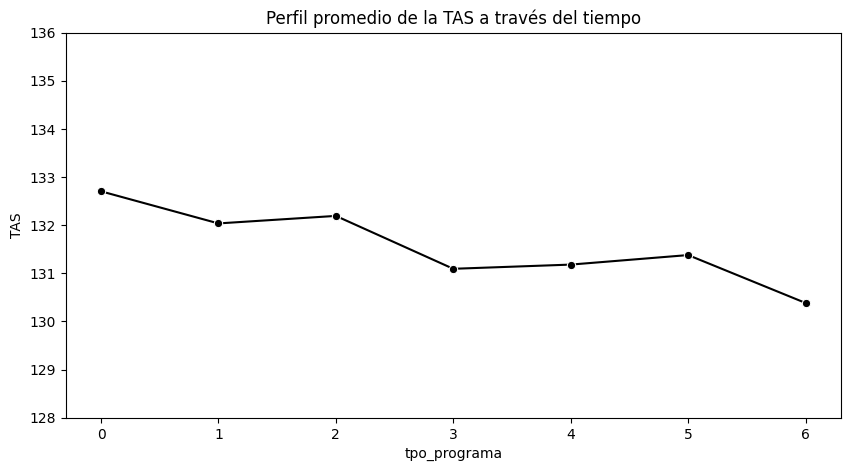
\includegraphics[scale=0.5]{img/TAS_vs_tpo.png}
	\caption{TAS de cada paciente en cada tiempo}
	\label{TAS_vs_tpo}
\end{figure}

En la figura \ref{spaghetti} se pueden observar las trayectorias individuales
de 15 pacientes seleccionados al azar, las pendientes son muy similares entre
sí, sin embargo hay variación en la ordenada al origen.

\begin{figure}[H]
	\centering
	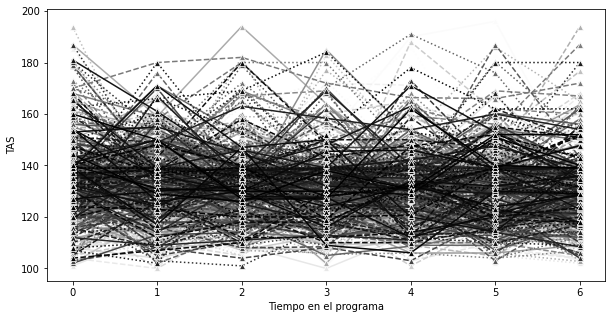
\includegraphics[scale=0.5]{img/spaghetti_plot.png}
	\caption{TAS a través del tiempo de 15 pacientes al azar}
	\label{spaghetti}
\end{figure}

Otro gráfico que resulta de interés es observar la evolución de la TAS a través
del tiempo pero sobre cada grupo de las covariables fijas, el resultado se
expresa en la figura \ref{TAS_with_covs}. Para las variables continuas, se
utilizó como punto de corte para segmentar en grupos la mediana de sus valores.
Podemos observar que en general la TAS disminuye, ya sea en mayor o menor
medida, a los largo del tiempo. Analizando las covariables de a una, el IMC
parece no tener un efecto significativo, dado que, aunque los pacientes con
menor IMC presentan menor TAS, los promedios en cada tiempo caen dentro de los
intervalos de confianza de ambos grupos. En cuanto a la edad y el sexo, no
parece haber una diferencia significativa en las pendientes pero si parece haber
una leve diferencia en las ordenadas al origen, presentando menor TAS los
pacientes más jóvenes y de sexo femenino. Por último, los pacientes con
antecedentes de diabetes parecen tener una TAS mayor en un comienzo con una
pendiente negativa a través del tiempo, mientras que los pacientes que no tienen
antecedentes de diabetes comienzan con una TAS mas inferior manteniendola más
constante.

\begin{figure}[H]
	\centering
	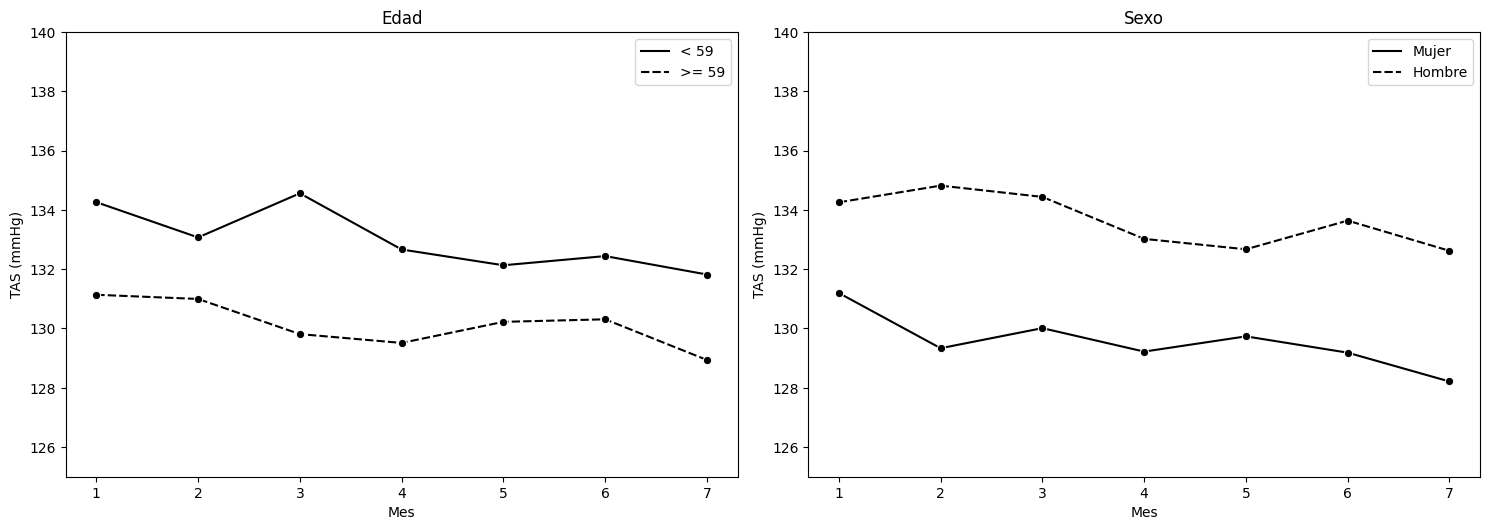
\includegraphics[scale=0.4]{img/TAS_vs_tpo_with_covs.png}
	\caption{TAS a través del tiempo según grupos de covariables}
	\label{TAS_with_covs}
\end{figure}

Por último, la figura \ref{TAS_with_adh} refleja el efecto de la adherencia al
tratamiento sobre la TAS. Para mantener perfiles no variables en el tiempo, se
usa la adherencia total al tratamiento y al igual que antes se divide en base a
su mediana, teniendo por un lado los pacientes que adhieren correctamente a más
del 86\% del tratamiento (al menos 6 de las 7 ocasiones) y por el otro a los
pacientes que adhieren correctamente menos del 86\% del tratamiento (hasta 5 de
las 7 ocasiones). Aqui se puede observar que los pacientes que adhieren
correctamente al tratamiento parecen tener una pendiente negativa en la TAS a
través del tiempo, mientras que los pacientes que no adhieren correctamente
mantienen la TAS más constante.

\begin{figure}[H]
	\centering
	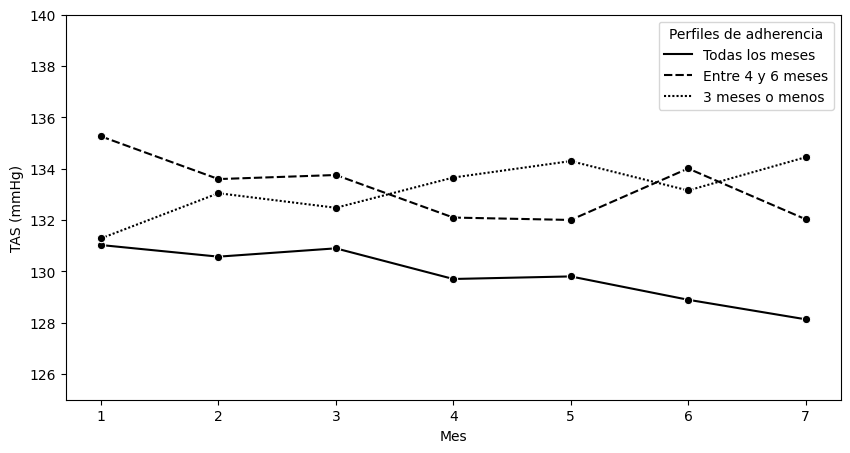
\includegraphics[scale=0.5]{img/TAS_vs_tpo_with_adherencia.png}
	\caption{TAS a través del tiempo según adherencia al tratamiento}
	\label{TAS_with_adh}
\end{figure}

\subsection{Evaluación de la exogeneidad}

Para evaluar la exogeneidad de la adherencia se ajustaron modelos de regresion
logística en cada ocasión, usando como variable respuesta la adherencia en dicha
ocasión y como covariables la TAS y la adherencia en la ocasión anterior y el
promedio y proporción hasta la ocasión anterior. En la tabla \ref{exog_table} se
presentan los valores de los coeficientes para cada covariable y en paréntesis
el p-value asociado a cada uno. Como se puede notar, en ninguna ocasión la
adherencia depende de valores anteriores de la TAS, por lo tanto puede
considerarse como una covariable exógena.

\begin{table}[H]
	\label{exog_table}
	\caption{Resultados de la prueba de exogeneidad}
	\begin{tabular}{*{5}{|c}|}
		\hline
		Ocasión\ (t) & $x_{t-1}$ & $\overline{x}_{t-2}$ & $y_{t-1}$ & $\overline{y}_{t-2}$ \\
		\hline
		\hline
		$1$ & $1.9302\ (<0.001)$ & $-$ & $0.0057\ (0.45)$ & $-$ \\
		$2$ & $2.3047\ (<0.001)$ & $0.5683\ (0.044)$ & $-0.0088\ (0.343)$ & $0.0075\ (0.419)$ \\
		$3$ & $1.9689\ (<0.001)$ & $1.0734\ (0.002)$ & $0.0138\ (0.17)$ & $-0.017\ (0.138)$ \\
		$4$ & $2.2945\ (<0.001)$ & $1.0617\ (0.007)$ & $0.0092\ (0.441)$ & $-0.0141\ (0.307)$ \\
		$5$ & $2.2741\ (<0.001)$ & $1.0698\ (0.015)$ & $-0.0008\ (0.938)$ & $<0.0001\ (0.996)$ \\
		$6$ & $2.5812\ (<0.001)$ & $1.4609\ (0.003)$ & $-0.0005\ (0.966)$ & $-0.0072\ (0.678)$ \\
		\hline
	\end{tabular}
\end{table}

\subsection{Modelo propuesto para la media}




\newpage
\nocite{*}
\renewcommand{\refname}{Bibliografía}
\bibliography{Bibliografia}

\end{document}